\documentclass[12pt,a4paper]{article}

% ─── Page Layout ───────────────────────────────────────────────────────────────
\usepackage[a4paper, margin=0.8in, headheight=14pt]{geometry}

% ─── Fonts (XeLaTeX) ───────────────────────────────────────────────────────────
\usepackage{fontspec}
\usepackage{unicode-math}
\setmainfont{TeX Gyre Pagella}
\setmonofont[Scale=0.88]{TeX Gyre Cursor}
\setmathfont{Latin Modern Math}

% ─── Packages ──────────────────────────────────────────────────────────────────
\usepackage{xcolor}
\usepackage{colortbl}
\usepackage{titlesec}
\usepackage{enumitem}
\usepackage{tabularx}
\usepackage{booktabs}
\usepackage{array}
\usepackage{amsmath}
\usepackage{tikz}
\usetikzlibrary{shapes.geometric, arrows.meta, positioning, calc, fit, decorations.pathreplacing}
\usepackage{tcolorbox}
\tcbuselibrary{skins, breakable}
\usepackage{hyperref}
\usepackage{fancyhdr}
\usepackage{graphicx}
\usepackage{microtype}
\hyphenpenalty=10000
\exhyphenpenalty=10000
\sloppy
\usepackage{caption}
\usepackage{setspace}
\usepackage{multirow}
\usepackage{tocloft}

% ─── Q&A helper ────────────────────────────────────────────────────────────────
\newcommand{\Q}[1]{\textbf{#1}\par\noindent\ignorespaces}

% ─── Colour Palette ────────────────────────────────────────────────────────────
\definecolor{myred}{RGB}{196,30,58}
\definecolor{mydark}{RGB}{30,30,50}
\definecolor{mygreen}{RGB}{14,120,80}
\definecolor{myteal}{RGB}{0,130,140}
\definecolor{myamber}{RGB}{180,100,0}
\definecolor{mypurple}{RGB}{100,30,160}
\definecolor{mygray}{RGB}{246,247,249}
\definecolor{mgframe}{RGB}{180,185,200}
\definecolor{watermark}{RGB}{145,150,170}
\definecolor{hdrred}{RGB}{250,232,235}
\definecolor{hdrgreen}{RGB}{220,244,233}
\definecolor{hdrteal}{RGB}{220,242,244}
\definecolor{hdramber}{RGB}{253,242,215}
\definecolor{hdrpurple}{RGB}{238,228,255}
\definecolor{hdrgray}{RGB}{238,240,245}
\definecolor{rowalt}{RGB}{250,251,253}

% ─── Section Formatting ────────────────────────────────────────────────────────
\titleformat{\section}
  {\large\bfseries\color{myred}}{\thesection.}{0.5em}{}
  [\vspace{1pt}{\color{myred}\rule{\linewidth}{0.8pt}}]
\titleformat{\subsection}
  {\normalsize\bfseries\color{myteal}}{\thesubsection}{0.5em}{}
\titlespacing*{\section}{0pt}{18pt}{7pt}
\titlespacing*{\subsection}{0pt}{11pt}{4pt}

% ─── Paragraph ─────────────────────────────────────────────────────────────────
\setlength{\parindent}{0pt}
\setlength{\parskip}{4pt}

% ─── TOC Styling ───────────────────────────────────────────────────────────────
\renewcommand{\cfttoctitlefont}{\large\bfseries\color{myred}}
\renewcommand{\cftaftertoctitle}{\par\noindent{\color{myred}\rule{\linewidth}{0.8pt}}}
\setlength{\cftbeforetoctitleskip}{0pt}
\setlength{\cftaftertoctitleskip}{6pt}
\renewcommand{\cftsecfont}{\normalsize\bfseries\color{mydark}}
\renewcommand{\cftsecpagefont}{\normalsize\bfseries\color{mydark}}
\renewcommand{\cftsecleader}{\cftdotfill{\cftdotsep}}
\setlength{\cftbeforesecskip}{7pt}
\renewcommand{\cftsubsecfont}{\small\color{mydark}}
\renewcommand{\cftsubsecpagefont}{\small\color{mydark}}
\setlength{\cftbeforesubsecskip}{3pt}
\setlength{\cftsubsecindent}{1.4em}

% ─── Table helpers ─────────────────────────────────────────────────────────────
\renewcommand{\arraystretch}{1.45}
\setlength{\tabcolsep}{6pt}
\arrayrulecolor{mydark}
\newcolumntype{B}[1]{>{\small\bfseries\raggedright\arraybackslash}m{#1}}
\newcolumntype{Y}{>{\small\raggedright\arraybackslash}X}
\renewcommand{\tabularxcolumn}[1]{m{#1}}

% ─── Header / Footer ───────────────────────────────────────────────────────────
\pagestyle{fancy}
\fancyhf{}
\fancyhead[L]{\small\color{myred}\textbf{HS-HU601}\;\color{mydark}--- Economics for Engineers}
\fancyhead[R]{\small\color{myteal}\textbf{Module 3 Notes}}
\fancyfoot[C]{\small\color{mydark}\thepage}
\fancyfoot[R]{\small\color{watermark}\textit{\copyright\ Biraj}}
\renewcommand{\headrulewidth}{0.5pt}
\renewcommand{\footrulewidth}{0.3pt}

% ─── Hyperref ──────────────────────────────────────────────────────────────────
\hypersetup{
  colorlinks=true, linkcolor=myteal, urlcolor=myteal,
  pdfauthor={Biraj Sarkar},
  pdftitle={HS-HU601 --- Module 3 Notes}
}

% ─── tcolorbox styles ──────────────────────────────────────────────────────────
\tcbset{
  tikzbox/.style={
    colback=mygray, colframe=mgframe, boxrule=0.6pt, arc=4pt,
    left=8pt, right=8pt, top=6pt, bottom=6pt,
    colbacktitle=mgframe, coltitle=mydark,
    fonttitle=\small\bfseries
  },
  defbox/.style={
    colback=hdrgreen, colframe=mygreen, boxrule=0.8pt, arc=4pt,
    left=9pt, right=9pt, top=6pt, bottom=6pt,
    colbacktitle=mygreen, coltitle=white,
    fonttitle=\small\bfseries
  },
  formulabox/.style={
    colback=hdrteal, colframe=myteal, boxrule=0.8pt, arc=4pt,
    left=9pt, right=9pt, top=7pt, bottom=7pt,
    colbacktitle=myteal, coltitle=white,
    fonttitle=\small\bfseries
  },
  examplebox/.style={
    colback=hdramber, colframe=myamber, boxrule=0.8pt, arc=4pt,
    left=9pt, right=9pt, top=6pt, bottom=6pt,
    colbacktitle=myamber, coltitle=white,
    fonttitle=\small\bfseries
  },
  masonbox/.style={
    colback=hdrpurple, colframe=mypurple, boxrule=0.8pt, arc=4pt,
    left=9pt, right=9pt, top=6pt, bottom=6pt,
    colbacktitle=mypurple, coltitle=white,
    fonttitle=\small\bfseries
  },
  exambox/.style={
    colback=hdrpurple, colframe=mypurple, boxrule=1pt, arc=5pt,
    left=10pt, right=10pt, top=8pt, bottom=8pt,
    colbacktitle=mypurple, coltitle=white,
    fonttitle=\bfseries,
    breakable, title after break={\textbf{Frequently Asked / Viva Questions (contd.)}}}
}
% Make all boxes breakable across pages
\tcbset{breakable}

% ─── TikZ styles ───────────────────────────────────────────────────────────────
\tikzset{
  block/.style={rectangle, draw=myteal, fill=hdrteal,
    text width=2.4cm, align=center, minimum height=0.95cm,
    font=\small, rounded corners=3pt, line width=0.7pt},
  redblock/.style={rectangle, draw=myred, fill=hdrred,
    text width=2.4cm, align=center, minimum height=0.95cm,
    font=\small, rounded corners=3pt, line width=0.7pt},
  arrow/.style={-Stealth, thick, color=mydark},
  redarrow/.style={-Stealth, thick, color=myred},
  line/.style={thick, color=mydark}
}

% ═══════════════════════════════════════════════════════════════════════════════
\begin{document}
% ═══════════════════════════════════════════════════════════════════════════════

\begin{center}
  {\LARGE\bfseries\color{myred} HS-HU601 --- Economics for Engineers}\\[5pt]
  {\normalsize\color{mydark} Semester VI \quad$\bullet$\quad 3L:0T:0P \quad$\bullet$\quad 3 Credits}\\[3pt]
  {\normalsize\color{myteal}\textbf{Module 3 Exam Notes}}\\[3pt]
  {\small\color{mydark} CGEC \;$|$\; B.Tech ECE (2023--27) \;$|$\; \textit{Biraj Sarkar}}
\end{center}
\vspace{2pt}
\noindent{\color{myred}\rule{\linewidth}{1.5pt}}
\vspace{2pt}

\hypersetup{linkcolor=mydark}
\tableofcontents
\hypersetup{linkcolor=myteal}
\newpage

% ===============================================================================
\section{Inflation and Price Change}
% ===============================================================================

Financial plans made in a stable environment can fail when prices rise over time.

\subsection{Inflation Concepts}
\begin{tcolorbox}[defbox]
\textbf{Inflation:} A general and progressive increase in the prices of goods and services over time, resulting in a decline in the purchasing power of money.
\par\vspace{3pt}
\textbf{Consumer Price Index (CPI):} A measure that examines the weighted average of prices of a basket of consumer goods and services. It is used to estimate price changes.
\end{tcolorbox}

\subsection{Interest Rates under Inflation (Fisher's Equation)}
Inflation separates the interest rate earned into a \textbf{nominal (market) rate} and a \textbf{real rate}.
\begin{itemize}[leftmargin=*, itemsep=4pt]
  \item \textbf{Nominal Interest Rate ($i$):} The actual interest rate paid or earned in the market.
  \item \textbf{Real Interest Rate ($i'$):} The interest rate adjusted to represent the real increase in purchasing power.
  \item \textbf{Inflation Rate ($f$):} The rate at which the price index increases.
\end{itemize}

\begin{tcolorbox}[formulabox, title={\textbf{Fisher's Equation}}]
The relationship between nominal interest, real interest, and inflation is:
\begin{equation}
  1 + i = (1 + i') \times (1 + f)
\end{equation}
Expanding this gives:
\begin{equation}
  i = i' + f + (i' \times f)
\end{equation}
To find the real interest rate:
\begin{equation}
  i' = \frac{i - f}{1 + f}
\end{equation}
\end{tcolorbox}

\subsection{Differential Inflation Rates}
Different components of a project (e.g., fuel, labor, equipment) may inflate at different rates. If a specific cost inflates at rate $f_j$, its future cash flow in year $t$ is:
\begin{equation}
  CF_t = CF_0 \times (1 + f_j)^t
\end{equation}
This is then discounted back to present using the market interest rate $i$.

% ===============================================================================
\section{Present Worth Analysis \& Mutual Exclusivity}
% ===============================================================================

When comparing competing engineering projects, specific conventions must be followed.

\subsection{Project Comparison Viewpoints}
1.  \textbf{Economic Studies Viewpoint:} Assesses the project based on total investment capital, ignoring how the project is financed.
2.  \textbf{Borrowed Money Viewpoint:} Includes the cash flows of borrowing (receipt of loan principal) and debt repayment (interest and principal payments).

\subsection{Effect of Income Taxes}
Corporate income taxes reduce net cash inflows.
\begin{itemize}[leftmargin=*, itemsep=4pt]
  \item $\text{Taxable Income} = \text{Revenues} - \text{Operating Expenses} - \text{Depreciation}$
  \item $\text{Income Tax} = \text{Taxable Income} \times \text{Corporate Tax Rate } (t)$
  \item \textbf{Tax Depreciation Shield:} Depreciation is a non-cash expense that reduces taxable income, shielding the company from taxes. The annual tax savings equal:
    \begin{equation}
      \text{Tax Shield} = t \times d_t \quad \text{($d_t$ is the depreciation in year $t$)}
    \end{equation}
\end{itemize}

\subsection{Comparing Projects with Unequal Lives}
We cannot compare the Present Worth of two alternatives directly if they have different useful lives because the service periods differ.
\begin{itemize}[leftmargin=*, itemsep=6pt]
  \item \textbf{Least Common Multiple (LCM) Method:} Compare projects over a study period equal to the LCM of their lives. It assumes that each alternative will be replaced at the end of its life with an identical asset at the same cost.
  \item \textbf{Co-termination (Study Period) Method:} A fixed study period is selected (e.g., 5 years). Any alternative with a shorter life is replaced, and any alternative with a longer life is assigned a salvage value at the end of the study period.
\end{itemize}

% ===============================================================================
\section{Uncertainty in Future Events}
% ===============================================================================

Engineering estimates of future costs and revenues are rarely certain.

\subsection{Expected Value}
When future cash flows are uncertain but can be assigned probabilities:
\begin{tcolorbox}[formulabox, title={\textbf{Expected Value Formula}}]
The expected value ($E[X]$) of a random cash flow variable $X$ is:
\begin{equation}
  E[X] = \sum_{j=1}^{M} x_j \times P(x_j)
\end{equation}
Where $x_j$ is the cash flow under outcome $j$, $P(x_j)$ is its probability, and $M$ is the number of outcomes.
\end{tcolorbox}

\subsection{Economic Decision Trees}
A decision tree is a graphical tool used to analyze decisions under risk.
\begin{itemize}[leftmargin=*, itemsep=4pt]
  \item \textbf{Decision Nodes (Squares):} Points where the decision-maker must select an alternative.
  \item \textbf{Chance Nodes (Circles):} Points where outcomes are determined by probability.
  \item \textbf{Branches:} Connect nodes; chance branches show probabilities and outcomes.
\end{itemize}

\begin{tcolorbox}[tikzbox, title={Economic Decision Tree for Plant Expansion}]
\centering
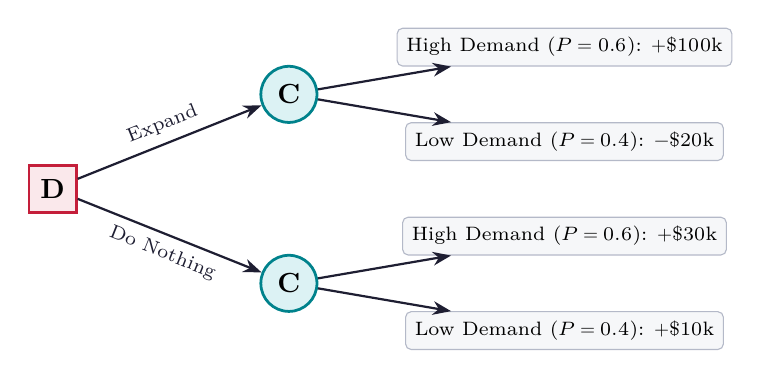
\begin{tikzpicture}[
  dnode/.style={rectangle, draw=myred, fill=hdrred, minimum size=0.6cm, line width=1.0pt},
  cnode/.style={circle, draw=myteal, fill=hdrteal, minimum size=0.6cm, line width=1.0pt},
  leaf/.style={rectangle, draw=mgframe, fill=mygray, font=\scriptsize, rounded corners=2pt},
  arrow/.style={-Stealth, thick, color=mydark}
]
  % Root Decision Node
  \node[dnode] (D1) at (0,0) {\textbf{D}};
  
  % Chance Nodes
  \node[cnode] (C1) at (3, 1.2) {\textbf{C}};
  \node[cnode] (C2) at (3, -1.2) {\textbf{C}};
  
  % Leaf Nodes
  \node[leaf] (L1) at (6.5, 1.8) {High Demand ($P=0.6$): $+\$100\text{k}$};
  \node[leaf] (L2) at (6.5, 0.6) {Low Demand ($P=0.4$): $-\$20\text{k}$};
  \node[leaf] (L3) at (6.5, -0.6) {High Demand ($P=0.6$): $+\$30\text{k}$};
  \node[leaf] (L4) at (6.5, -1.8) {Low Demand ($P=0.4$): $+\$10\text{k}$};
  
  % Connect D1 to C1 and C2
  \draw[arrow] (D1) -- node[above, sloped, font=\scriptsize] {Expand} (C1);
  \draw[arrow] (D1) -- node[below, sloped, font=\scriptsize] {Do Nothing} (C2);
  
  % Connect C1 to L1, L2
  \draw[arrow] (C1) -- (L1);
  \draw[arrow] (C1) -- (L2);
  
  % Connect C2 to L3, L4
  \draw[arrow] (C2) -- (L3);
  \draw[arrow] (C2) -- (L4);
\end{tikzpicture}
\end{tcolorbox}

% ===============================================================================
\section{Worked Examples}
% ===============================================================================

\begin{tcolorbox}[examplebox, title={Example 1: Fisher's Equation}]
\textbf{Problem:} An electronics engineer wants to earn a real rate of return of $6\%$ per year on an investment. If inflation is projected to run at an average rate of $4\%$ per year over the next few years, what nominal market interest rate must the investment yield?\\[4pt]
\textbf{Solution:}
Identify given parameters: Real interest rate $i' = 0.06$, Inflation rate $f = 0.04$.
Using Fisher's Equation:
\begin{align*}
  i &= i' + f + (i' \times f) \\
  i &= 0.06 + 0.04 + (0.06 \times 0.04) \\
  i &= 0.10 + 0.0024 \\
  i &= 0.1024 = 10.24\%
\end{align*}
\textbf{Alternative check using $(1+i)$:}
\begin{align*}
  1 + i &= (1 + i')(1 + f) = (1.06) \times (1.04) = 1.1024 \quad \Rightarrow \quad i = 10.24\%
\end{align*}
\textbf{Answer:} The investment must yield a nominal market interest rate of \textbf{10.24\%}.
\end{tcolorbox}

\begin{tcolorbox}[examplebox, title={Example 2: Mutually Exclusive Projects with Unequal Lives}]
\textbf{Problem:} Compare two manufacturing machines at an interest rate of $10\%$ using the Present Worth method.
\begin{itemize}[leftmargin=*, itemsep=3pt, topsep=2pt]
  \item \textbf{Machine A:} Initial cost $= \$10,000$, useful life $= 2$ years, annual operating cost $= \$2,000$.
  \item \textbf{Machine B:} Initial cost $= \$15,000$, useful life $= 3$ years, annual operating cost $= \$1,500$.
\end{itemize}
\vspace{4pt}
\textbf{Solution:}
The lives are unequal ($2$ and $3$ years). The study period must be the Least Common Multiple:
\begin{equation*}
  \text{Study Period} = \text{LCM}(2, 3) = 6 \text{ years}
\end{equation*}
\begin{itemize}[leftmargin=*, itemsep=8pt]
  \item \textbf{Machine A (re-purchased at end of Year 2 and Year 4):} \\
    Cash outflows occur at $t=0$ ($\$10\text{k}$), $t=2$ ($\$10\text{k}$), $t=4$ ($\$10\text{k}$), and annual costs of $\$2\text{k}$ for Years $1..6$.
    \begin{align*}
      PW_A(10\%) &= -10,000 - 10,000 \times (P/F, 10\%, 2) - 10,000 \times (P/F, 10\%, 4) \\
                 & \quad - 2,000 \times (P/A, 10\%, 6) \\
      PW_A(10\%) &= -10,000 - 10,000(0.8264) - 10,000(0.6830) - 2,000(4.3553) \\
      PW_A(10\%) &= -10,000 - 8,264 - 6,830 - 8,711 = -\$33,805
    \end{align*}
  \item \textbf{Machine B (re-purchased at end of Year 3):} \\
    Cash outflows occur at $t=0$ ($\$15\text{k}$), $t=3$ ($\$15\text{k}$), and annual costs of $\$1.5\text{k}$ for Years $1..6$.
    \begin{align*}
      PW_B(10\%) &= -15,000 - 15,000 \times (P/F, 10\%, 3) - 1,500 \times (P/A, 10\%, 6) \\
      PW_B(10\%) &= -15,000 - 15,000(0.7513) - 1,500(4.3553) \\
      PW_B(10\%) &= -15,000 - 11,270 - 6,533 = -\$32,803
    \end{align*}
\end{itemize}
Comparing the Present Worths over 6 years:
\begin{align*}
  PW_B (-\$32,803) &> PW_A (-\$33,805) \quad (\text{Machine B has lower net present cost})
\end{align*}
\textbf{Answer:} \textbf{Machine B} is selected since it minimizes the net present cost over the 6-year study period.
\end{tcolorbox}

\begin{tcolorbox}[examplebox, title={Example 3: Decision Tree Rollback}]
\textbf{Problem:} Roll back the plant expansion decision tree shown in Section 3.2. Find the expected value for each alternative and determine the optimal decision.\\[4pt]
\textbf{Solution:}
Calculate the Expected Value (EV) for each decision branch:
1.  \textbf{Branch 1: Expand}
    The outcomes are High Demand ($+\$100\text{k}$ at $P=0.6$) and Low Demand ($-\$20\text{k}$ at $P=0.4$).
    \begin{align*}
      EV(\text{Expand}) &= 100,000 \times 0.6 + (-20,000) \times 0.4 \\
                        &= 60,000 - 8,000 = \$52,000
    \end{align*}
2.  \textbf{Branch 2: Do Nothing}
    The outcomes are High Demand ($+\$30\text{k}$ at $P=0.6$) and Low Demand ($+\$10\text{k}$ at $P=0.4$).
    \begin{align*}
      EV(\text{Do Nothing}) &= 30,000 \times 0.6 + 10,000 \times 0.4 \\
                            &= 18,000 + 4,000 = \$22,000
    \end{align*}
Compare expected values at the root decision node:
\begin{align*}
  EV(\text{Expand}) = \$52,000 &> EV(\text{Do Nothing}) = \$22,000
\end{align*}
The optimal choice is to select the path with the highest expected value.
\par\vspace{3pt}
\textbf{Answer:} The optimal decision is to \textbf{Expand}, with an expected value of \textbf{\$52,000}.
\end{tcolorbox}

% ===============================================================================
% MANDATORY QUICK REVISION PAGE
% ===============================================================================
\newpage
\begin{center}
  {\large\bfseries\color{myred} Quick Revision --- Module III}\\[3pt]
  {\small\color{mydark} Inflation, Present Worth \& Uncertainty $|$ HS-HU601}
\end{center}
\noindent{\color{myred}\rule{\linewidth}{1.2pt}}
\vspace{4pt}

\begin{tcolorbox}[formulabox, title={\textbf{Key Formulas at a Glance}}]
\renewcommand{\arraystretch}{1.3}
\begin{tabularx}{\linewidth}{B{3.8cm} X}
Fisher's Equation       & $i = i' + f + i'f$ \\[4pt]
Real Interest Rate      & $i' = \displaystyle\frac{i - f}{1 + f}$ \\[6pt]
Tax Depreciation Shield & $\text{Tax Savings} = t \times d_t$ \quad ($t$ = tax rate, $d_t$ = depreciation) \\[4pt]
Expected Value          & $E[X] = \displaystyle\sum x_j P(x_j)$ \\[6pt]
LCM Study Period        & Study Period = Least Common Multiple of individual project lives
\end{tabularx}
\end{tcolorbox}

\begin{tcolorbox}[defbox, title={\textbf{One-Line Definitions}}]
\begin{itemize}[leftmargin=*, itemsep=2pt, topsep=0pt]
  \item \textbf{CPI:} An index measuring inflation by tracking average price changes of consumer goods.
  \item \textbf{Real Interest Rate:} The rate of return adjusted to reflect actual increases in purchasing power.
  \item \textbf{Tax Shield:} The reduction in income tax liability resulting from tax-deductible depreciation.
  \item \textbf{LCM Method:} Project comparison method over a study period matching the least common multiple of their lives.
  \item \textbf{Co-termination:} Comparing alternatives over a fixed study period, assigning salvage value to remaining assets.
  \item \textbf{Expected Value:} Weighted average of all possible numerical outcomes, using probabilities as weights.
  \item \textbf{Decision Tree:} Graphical model displaying sequential decisions, probabilities, and financial outcomes.
  \item \textbf{Monte Carlo Simulation:} Computational algorithm that uses repeated random sampling to model uncertainty.
\end{itemize}
\end{tcolorbox}

\begin{tcolorbox}[exambox, title={\textbf{Frequently Asked / Viva Questions}}]
\begin{enumerate}[topsep=0pt, label=\textbf{Q\arabic*.}, itemsep=5pt]
  \item \Q{How does inflation affect the value of cash flows over time?}
    Inflation reduces the purchasing power of money, meaning future cash flows are worth less in real terms than nominal terms.
  \item \Q{State Fisher's Equation and define its variables.}
    $i = i' + f + i'f$, where $i$ is the nominal market interest rate, $i'$ is the real interest rate, and $f$ is the inflation rate.
  \item \Q{What is the difference between the economic studies and borrowed money viewpoints?}
    Economic studies viewpoint evaluates a project based on total capital requirements, ignoring financing. Borrowed money viewpoint includes the loan receipts and debt payments.
  \item \Q{How does depreciation act as a tax shield?}
    Depreciation is a non-cash expense that is subtracted from revenue to calculate taxable income. By lowering taxable income, it reduces corporate tax liability.
  \item \Q{Why can we not compare PW of unequal-life alternatives directly?}
    Because the alternatives do not provide service over the same timeframe. Comparing them directly over different lives violates the equal-service comparison rule.
  \item \Q{Describe the assumption behind the Least Common Multiple (LCM) method.}
    It assumes that each alternative can be replaced at the end of its life with an identical asset having the same initial cost and operating costs.
  \item \Q{Explain the co-termination method for comparing unequal-life projects.}
    A specific study period is chosen. Shorter-lived alternatives are replaced, and longer-lived alternatives are terminated early, assigning them a salvage value.
  \item \Q{What is the difference between decision nodes and chance nodes in a decision tree?}
    Decision nodes (squares) represent points where the engineer has control over choices. Chance nodes (circles) represent points where outcomes occur based on probability.
  \item \Q{How do we roll back (solve) a decision tree?}
    We work from right to left (backwards). At each chance node, we calculate the expected value. At each decision node, we select the branch with the highest value.
  \item \Q{What does a high risk-premium imply for a project's MARR?}
    High-risk projects require a higher risk-premium, which increases the Minimum Attractive Rate of Return (MARR) used to discount its cash flows.

  \item \Q{What is the purpose of Monte Carlo simulation in risk analysis?}
    It allows the engineer to model parameters as probability distributions rather than single-point estimates, generating a distribution of possible PW outcomes.
  \item \Q{What are Real Options in engineering project management?}
    The managerial flexibility to adapt decisions in response to market changes, such as the option to expand, contract, defer, or abandon a project.
\end{enumerate}
\end{tcolorbox}

\begin{tcolorbox}[tikzbox, title={Comparison of Project Selection Methods under Equivalence}]
\renewcommand{\arraystretch}{1.45}
\par\noindent
\begin{tabularx}{\linewidth}{|B{2.3cm}|Y|Y|Y|}
\hline
\textbf{Method} & \textbf{Core Metric} & \textbf{Study Period Rule} & \textbf{Primary Application} \\
\hline
\textbf{Present Worth (PW)} & Net present value at $t=0$ & Must be equal (use LCM for unequal lives) & Comparing mutually exclusive projects with defined lives. \\
\hline
\textbf{Annual Worth (AW)} & Equivalent uniform annual series & Equal to useful life (does not require LCM) & Comparing alternatives with unequal service lives easily. \\
\hline
\textbf{IRR} & Discount rate where $PW = 0$ & Compare IRR to MARR; requires incremental analysis & Evaluating single projects or ranking capital budgets. \\
\hline
\textbf{BCR} & Ratio of discounted benefits to costs & Equal study period required & Public sector projects and government infrastructure. \\
\hline
\end{tabularx}
\end{tcolorbox}

\end{document}
